\documentclass{beamer}
\usetheme{default}
\usecolortheme{seahorse}
\usepackage[utf8]{inputenc}
\usepackage{graphicx}
\usepackage{booktabs}
\usepackage{amsmath}
\usepackage{natbib}
\usepackage[italian]{babel}
\usepackage{hyphenat}
\hyphenation{mate-mati-ca recu-perare}
\usepackage{tikz}
\usetikzlibrary{shapes,arrows.meta,positioning}

\title[Lezione 4]{Modelli ad Equazioni Strutturali}
\subtitle{Master Avanzato in Economia e Politica Agraria}
\author{Giovanbattista Califano}
\date[Portici, 30/04/2026]{Scale Attitudinali per lo Studio \\ delle Preferenze del Consumatore \\ 30 Aprile e 7 Maggio 2026}
\institute[UNINA]{Università degli Studi di Napoli Federico II, giovanbattista.califano@unina.it}

\tikzset{
  lv/.style = {draw=blue!80, fill=blue!10, very thick, ellipse, minimum height=1cm, minimum width=2cm, align=center}, 
  mv/.style = {draw=blue!80, fill=blue!10, very thick, rectangle, minimum height=0.5cm, minimum width=1cm, align=center}, 
  ev/.style = {draw=blue!80, fill=blue!10, very thick, circle, minimum size=0.6cm, inner sep=1pt, align=center}, 
  arrow/.style = {thick, ->, >=Stealth}
}

\AtBeginSection[]
{
  \begin{frame}<beamer>
    \frametitle{Passiamo a...}
    \tableofcontents[currentsection]
  \end{frame}
}

\begin{document}

\frame{\titlepage}

\begin{frame}{Tabella di marcia}
    \begin{center}
        \begin{tabular}{|l|l|c|}
        \hline
        20/04 e 23/04 &  Hello, Psychometrics! & $\checkmark$ \\
        \hline
        24/04 & Affidabilità e Validità di una Misura & $\checkmark$ \\
        \hline
        24/04 e 27/04 & Variabili Latenti: Riflessive o Formative? & $\checkmark$ \\
        \hline
        30/04 e 07/05 & Modelli ad Equazioni Strutturali & $\bigcirc$ \\
        \hline
        \end{tabular}
    \end{center}
\vspace{0.1cm}
\footnotesize
Riferimenti consigliati: \\
\begin{itemize}
    \item Capitoli 4 e 7 da \cite{jhangiani2019research}
    \item Capitoli 7, 10 e 14 da \cite{olivero2022psicologia}
    \item Capitolo 12 da \cite{mehmetoglu2022applied}
\end{itemize}
\scriptsize
\bibliographystyle{apalike}
\bibliography{text}
\end{frame}

\begin{frame}{Esame}
    A ciascuno di voi è stato assegnato un articolo scientifico. L’obiettivo dell’esame è analizzare criticamente l’uso degli strumenti psicometrici all’interno dello studio e proporre un’estensione motivata, fondata sulle vostre conoscenze teoriche e metodologiche. Il report va consegnato entro il \textbf{27/06/2025}. \\
    \vspace{1em}
    Info e materiale: \\
    \url{https://data.califano.xyz/esame}
\end{frame}

\begin{frame}{Prima di iniziare...}
    \centering
    \url{https://www.stata.com/manuals/sem.pdf}
\end{frame}

\begin{frame}{Prima di iniziare...}
    \begin{figure}
        \centering
        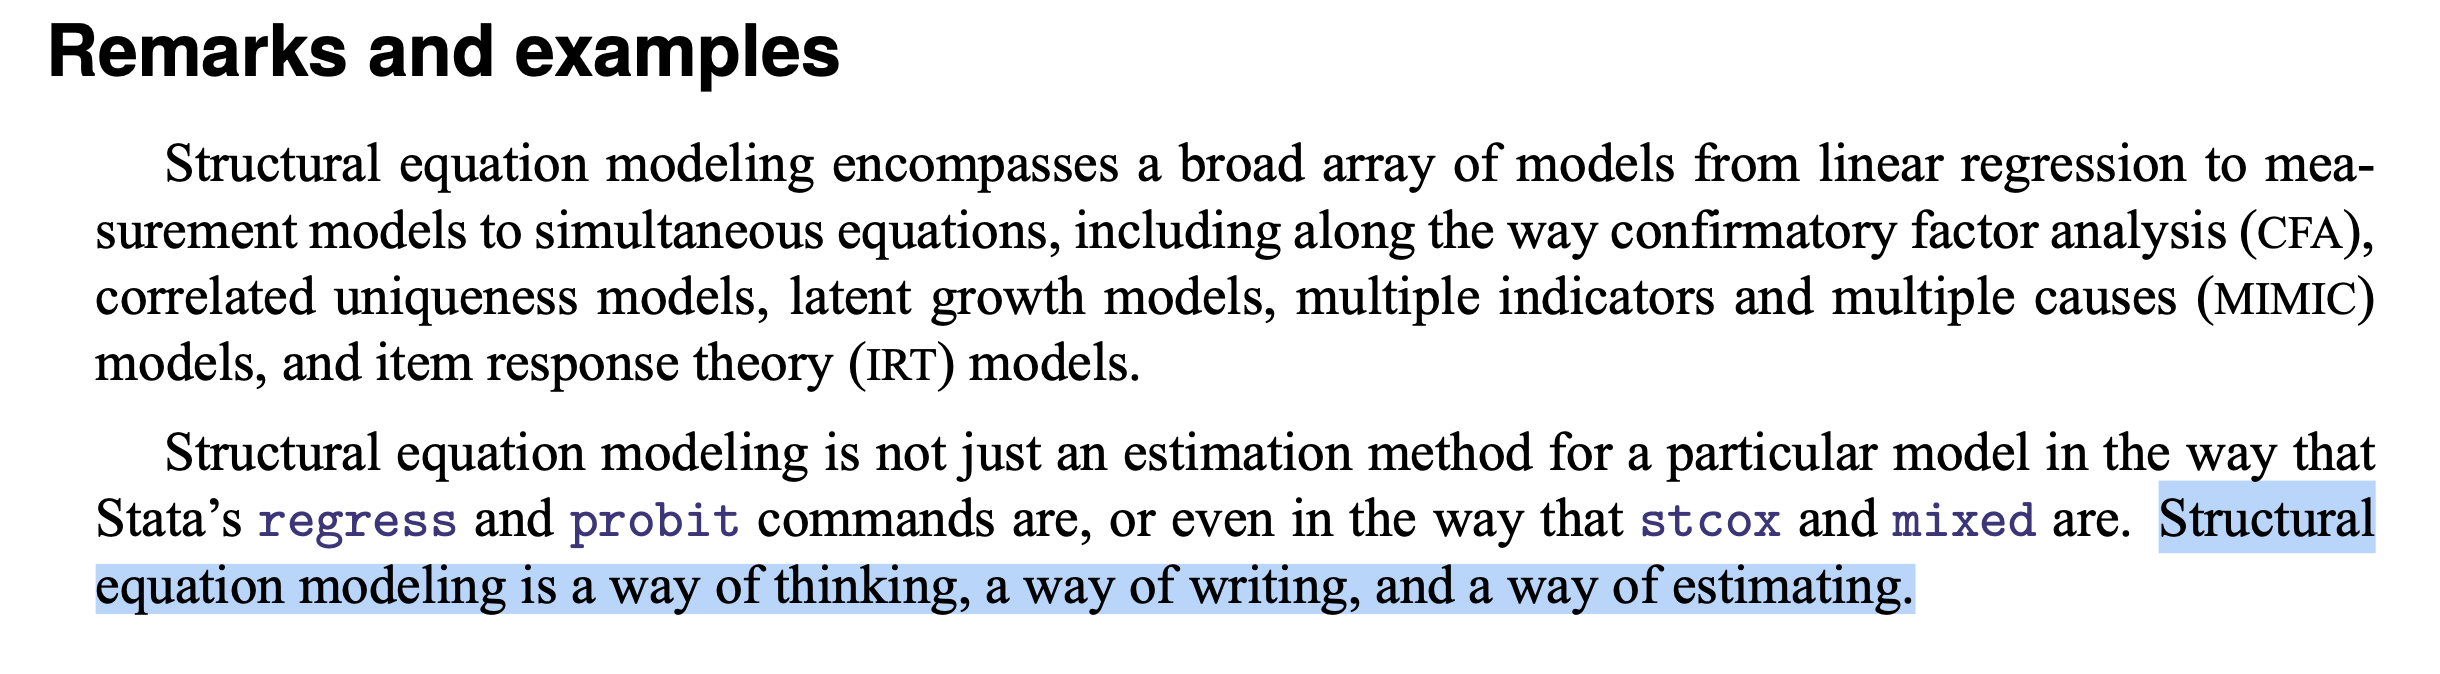
\includegraphics[width=1\linewidth]{manual.png}
    \end{figure}
    \centering
    \pause
    \begin{tikzpicture}[node distance=0.3 and 1.5, auto]
        \node[mv] (x) {$x$};
        \node[mv, right=of x] (y) {$y$};
        \node[ev, right=0.5 of y] (e) {$\varepsilon$};
        \draw[arrow] (x) -- (y);
        \draw[arrow] (e) -- (y);
    \end{tikzpicture}
\end{frame}

\begin{frame}{Prima di iniziare...}
    \begin{figure}
        \centering
        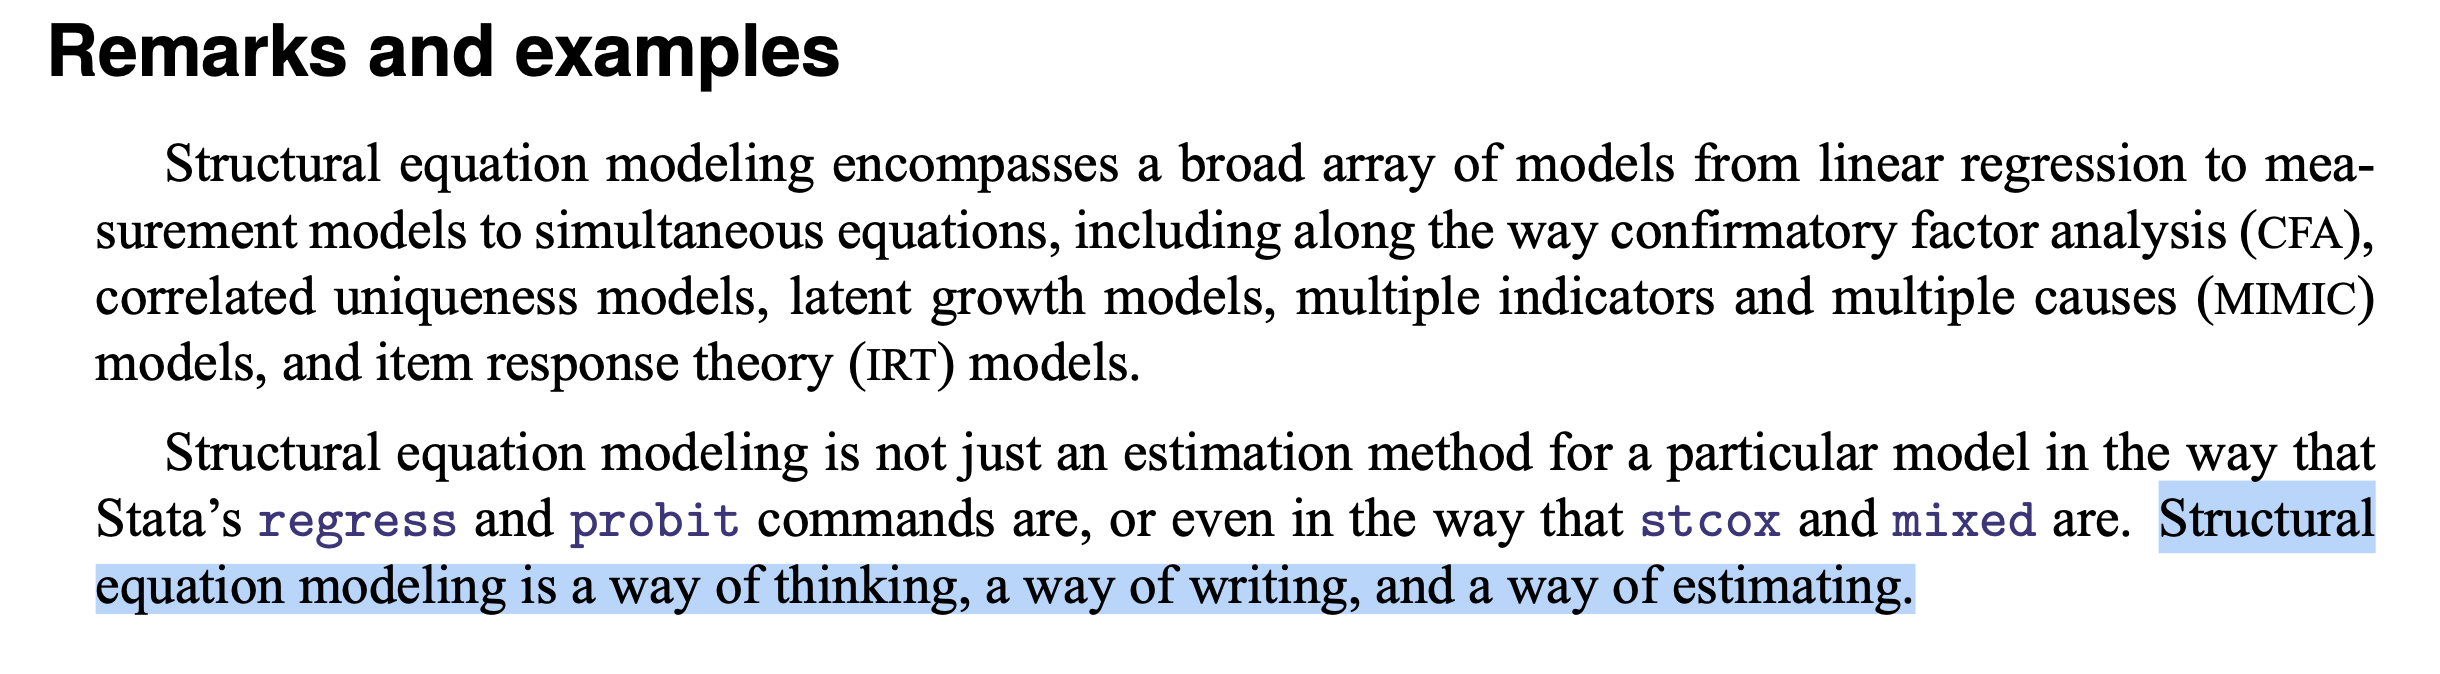
\includegraphics[width=1\linewidth]{manual.png}
    \end{figure}
    \centering
    \begin{tikzpicture}[node distance=0.3 and 1.5, auto]
        \node[mv] (x1) {$x_1$};
        \node[mv, below=of x1] (x2) {$x_2$};
        \node[mv, below=of x2] (x3) {$x_3$};
        \node[mv, below=of x3] (x4) {$x_4$};
        \node[mv, right=of x2] (y1) {$y_1$};
        \node[mv, right=of x3] (y2) {$y_2$};
        \node[ev, right=0.5 of y1] (e1) {$\varepsilon_1$};
        \node[ev, right=0.5 of y2] (e2) {$\varepsilon_2$};
        \draw[arrow] (x1) -- (y1);
        \draw[arrow] (x2) -- (y1);
        \draw[arrow] (x3) -- (y1);
        \draw[arrow] (x3) -- (y2);
        \draw[arrow] (x4) -- (y2);
        \draw[arrow] (e1) -- (y1);
        \draw[arrow] (e2) -- (y2);
        \draw[<->, thick, >=Stealth] (e1.east) to [out=10,in=10] (e2.east);
    \end{tikzpicture}
\end{frame}

\section{Un po' di terminologia}
\begin{frame}{Tipi di SEM}
    \begin{itemize}
        \item La modellistica a equazioni strutturali permette di stimare le relazioni tra variabili osservate e/o latenti attraverso lo studio della matrice di varianza e covarianza. Per questo, è anche chiamata \textbf{Covariance Based (CB) SEM}\footnote{Anche per distinguerla dalla Partial Least Squares (PLS) SEM.}.
        \item Poiché viene utilizzata per stimare più equazioni simultaneamente, i modelli sono descritti e riportati in forma di diagrammi a blocchi.
        \item Come notava anche il buon manuale di Stata, sotto il cappello della SEM rientrano molti modelli diversi...
    \end{itemize}
\end{frame}

\begin{frame}{Qualche esempio}
    \centering
    \textbf{Path Analysis (PA)} \\
    \vspace{2em}
    \begin{columns}
        \column{0.5\textwidth}
        \begin{tikzpicture}
            \node[mv] (y) {$y$};
            \node[mv, left=of y] (m) {$m$};
            \node[mv, left=of m] (x) {$x$};
            \draw[arrow] (x) -- (m);
            \draw[arrow] (m) -- (y);        
        \end{tikzpicture}
        \column{0.5\textwidth}
        \begin{tikzpicture}
            \node[mv] (y) {$y$};
            \node[left=of y] (dummy) {};
            \node[mv, above=of dummy] (m) {$m$};
            \node[mv, left=of dummy] (x) {$x$};
            \draw[arrow] (x) -- (m);
            \draw[arrow] (m) -- (y);
            \draw[arrow] (x) -- (y);
        \end{tikzpicture}
    \end{columns}
    \vspace{2em} \\
    \textit{Si stimano relazioni tra variabili manifeste.}
\end{frame}

\begin{frame}{Qualche esempio}
    \centering
    \textbf{Path Analysis (PA)} \\
    \vspace{2em}
        \begin{tikzpicture}
            \node[mv] (y) {Endogena};
            \node[left=of y] (dummy) {};
            \node[mv, above=of dummy] (m) {Endogena};
            \node[mv, left=of dummy] (x) {Esogena};
            \draw[arrow] (x) -- (m);
            \draw[arrow] (m) -- (y);
            \draw[arrow] (x) -- (y);
        \end{tikzpicture}
    \vspace{2em} \\
    \textit{In questi modelli è complicato parlare di variabili dipendenti e indipendenti. Le variabili che non sono spiegate nel modello si definiscono esogene, mentre quelle che vengono spiegate si definiscono endogene.}
\end{frame}

\begin{frame}{Qualche esempio}
    \centering
    \textbf{Confirmatory Factor Analysis (CFA)} \\
    \vspace{2em}
        \begin{tikzpicture}
            \node[lv] (l) {$\eta$};
            \node[mv, left=of l] (x2) {$y_2$};
            \node[mv, above=of x2] (x1) {$y_1$};
            \node[mv, below=of x2] (x3) {$y_3$};
            \draw[arrow] (l) -- (x1);
            \draw[arrow] (l) -- (x2);
            \draw[arrow] (l) -- (x3);
        \end{tikzpicture}
    \vspace{2em} \\
    \textit{Si stimano relazioni tra variabili manifeste e latenti.}
\end{frame}

\begin{frame}{Qualche esempio}
    \centering
    \textbf{Latent Path Analysis (LPA)} \\
    \vspace{2em}
        \begin{tikzpicture}
            \node[lv] (et) {$\eta$};
            \node[lv, left=of et] (xi) {$\xi$};
            \draw[arrow] (xi) -- (et);
        \end{tikzpicture}
    \vspace{2em} \\
    \textit{Si stimano relazioni tra variabili latenti.}
\end{frame}

\begin{frame}{Qualche esempio}
    \centering
    \textbf{CFA + LPA} \\
    \textit{Ciò che si intende comunemente con SEM} \\
    \vspace{2em}
        \begin{tikzpicture}
            \node[lv] (et) {$\eta$};
            \node[lv, left=2 of et] (xi) {$\xi$};
            \node[mv, left=of xi] (x2) {$x_2$};
            \node[mv, above=of x2] (x1) {$x_1$};
            \node[mv, below=of x2] (x3) {$x_3$};
            \node[mv, right=of et] (y2) {$y_2$};
            \node[mv, above=of y2] (y1) {$y_1$};
            \node[mv, below=of y2] (y3) {$y_3$};
            \draw[arrow] (xi) -- (et);
            \draw[arrow] (xi) -- (x1);
            \draw[arrow] (xi) -- (x2);
            \draw[arrow] (xi) -- (x3);
            \draw[arrow] (et) -- (y1);
            \draw[arrow] (et) -- (y2);
            \draw[arrow] (et) -- (y3);
        \end{tikzpicture}
    \vspace{2em} \\
    \small
    \textit{In questi casi la parte di CFA viene definita come \textbf{modello di misurazione} o \textbf{modello esterno} (outer). La parte di LPA (o PA), invece, come \textbf{modello strutturale} o \textbf{modello interno} (inner).}
\end{frame}

\begin{frame}{Qualche esempio}
    \centering
    \textbf{Le variabili latenti sono solo continue?} \\
    \vspace{2em}
        \begin{tikzpicture}
            \node[lv] (l) {$C$};
            \node[mv, left=of l] (x2) {$y_5$};
            \node[mv, above=of x2] (x1) {$y_4$};
            \node[mv, below=of x2] (x3) {$y_6$};
            \draw[arrow] (l) -- (x1);
            \draw[arrow] (l) -- (x2);
            \draw[arrow] (l) -- (x3);
        \end{tikzpicture}
    \vspace{2em} \\
    \textit{No. Possiamo ipotizzare l'esistenza di classi non osservabili (o non osservate) e stimarle a partire da indicatori osservati. SEM a variabili latenti categoriali includono Latent Class Analysis, Latent Profile Analysis, e altri modelli di misture finite.}
\end{frame}

\section{Un po' di storia}
\begin{frame}{Breve storia della SEM}
    \small
    \begin{block}{Origini}
        L'analisi SEM nasce dall'integrazione di:
        \begin{itemize}
            \item \textbf{Path Analysis} (Sewall Wright, 1921)
            \item \textbf{Analisi Fattoriale} (Spearman, 1904; Thurstone, 1930)
            \item \textbf{Modelli a variabili latenti} (Jöreskog, 1969)
        \end{itemize}
        \vspace{0.5em}
        La SEM unifica approcci di tipo causale e misurativo in un'unica struttura statistica.
    \end{block}
    \begin{columns}[c]
    \column{0.25\textwidth}
    \begin{figure}
        \centering
        \footnotesize\textbf{Sewall Wright} \\
        \vspace{0.2em}
        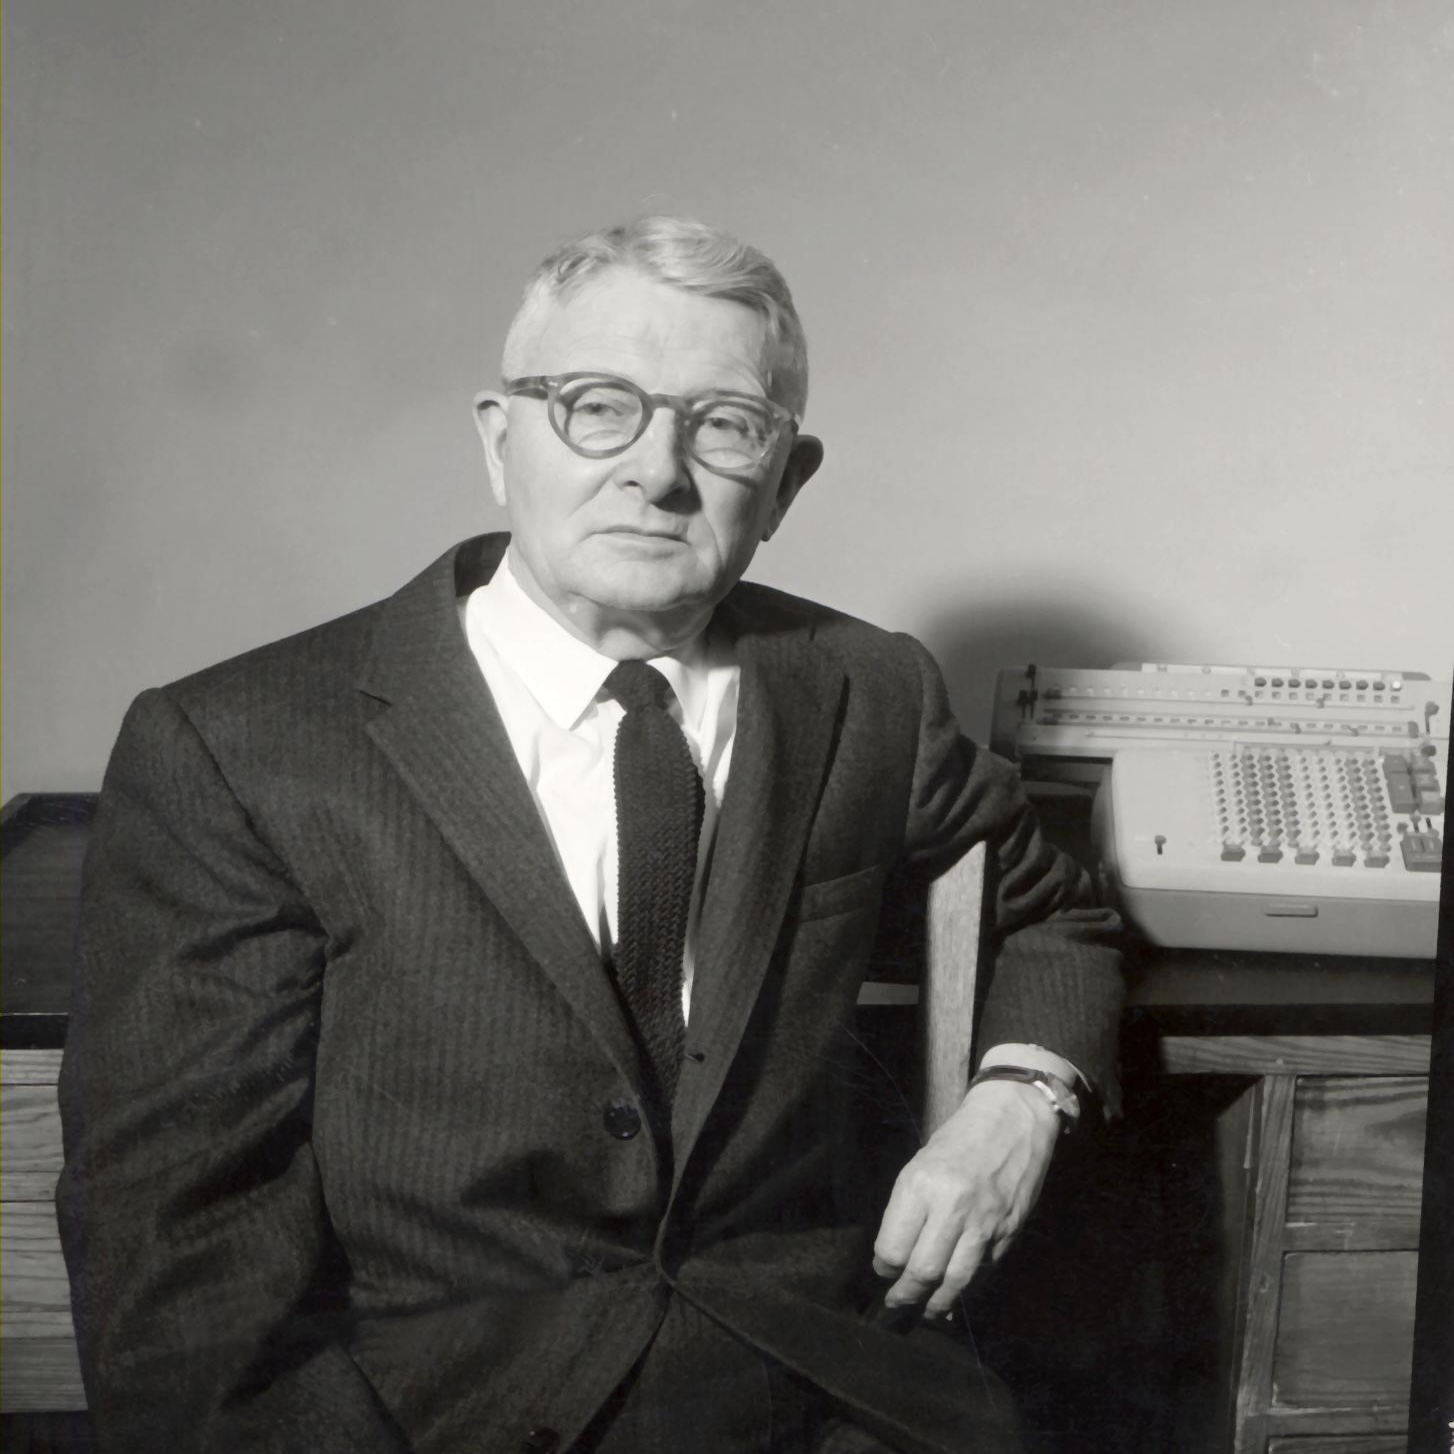
\includegraphics[width=\linewidth]{_wright.jpg}
    \end{figure}
    \column{0.25\textwidth}
    \begin{figure}
        \centering
        \footnotesize\textbf{Charles Spearman} \\
        \vspace{0.2em}
        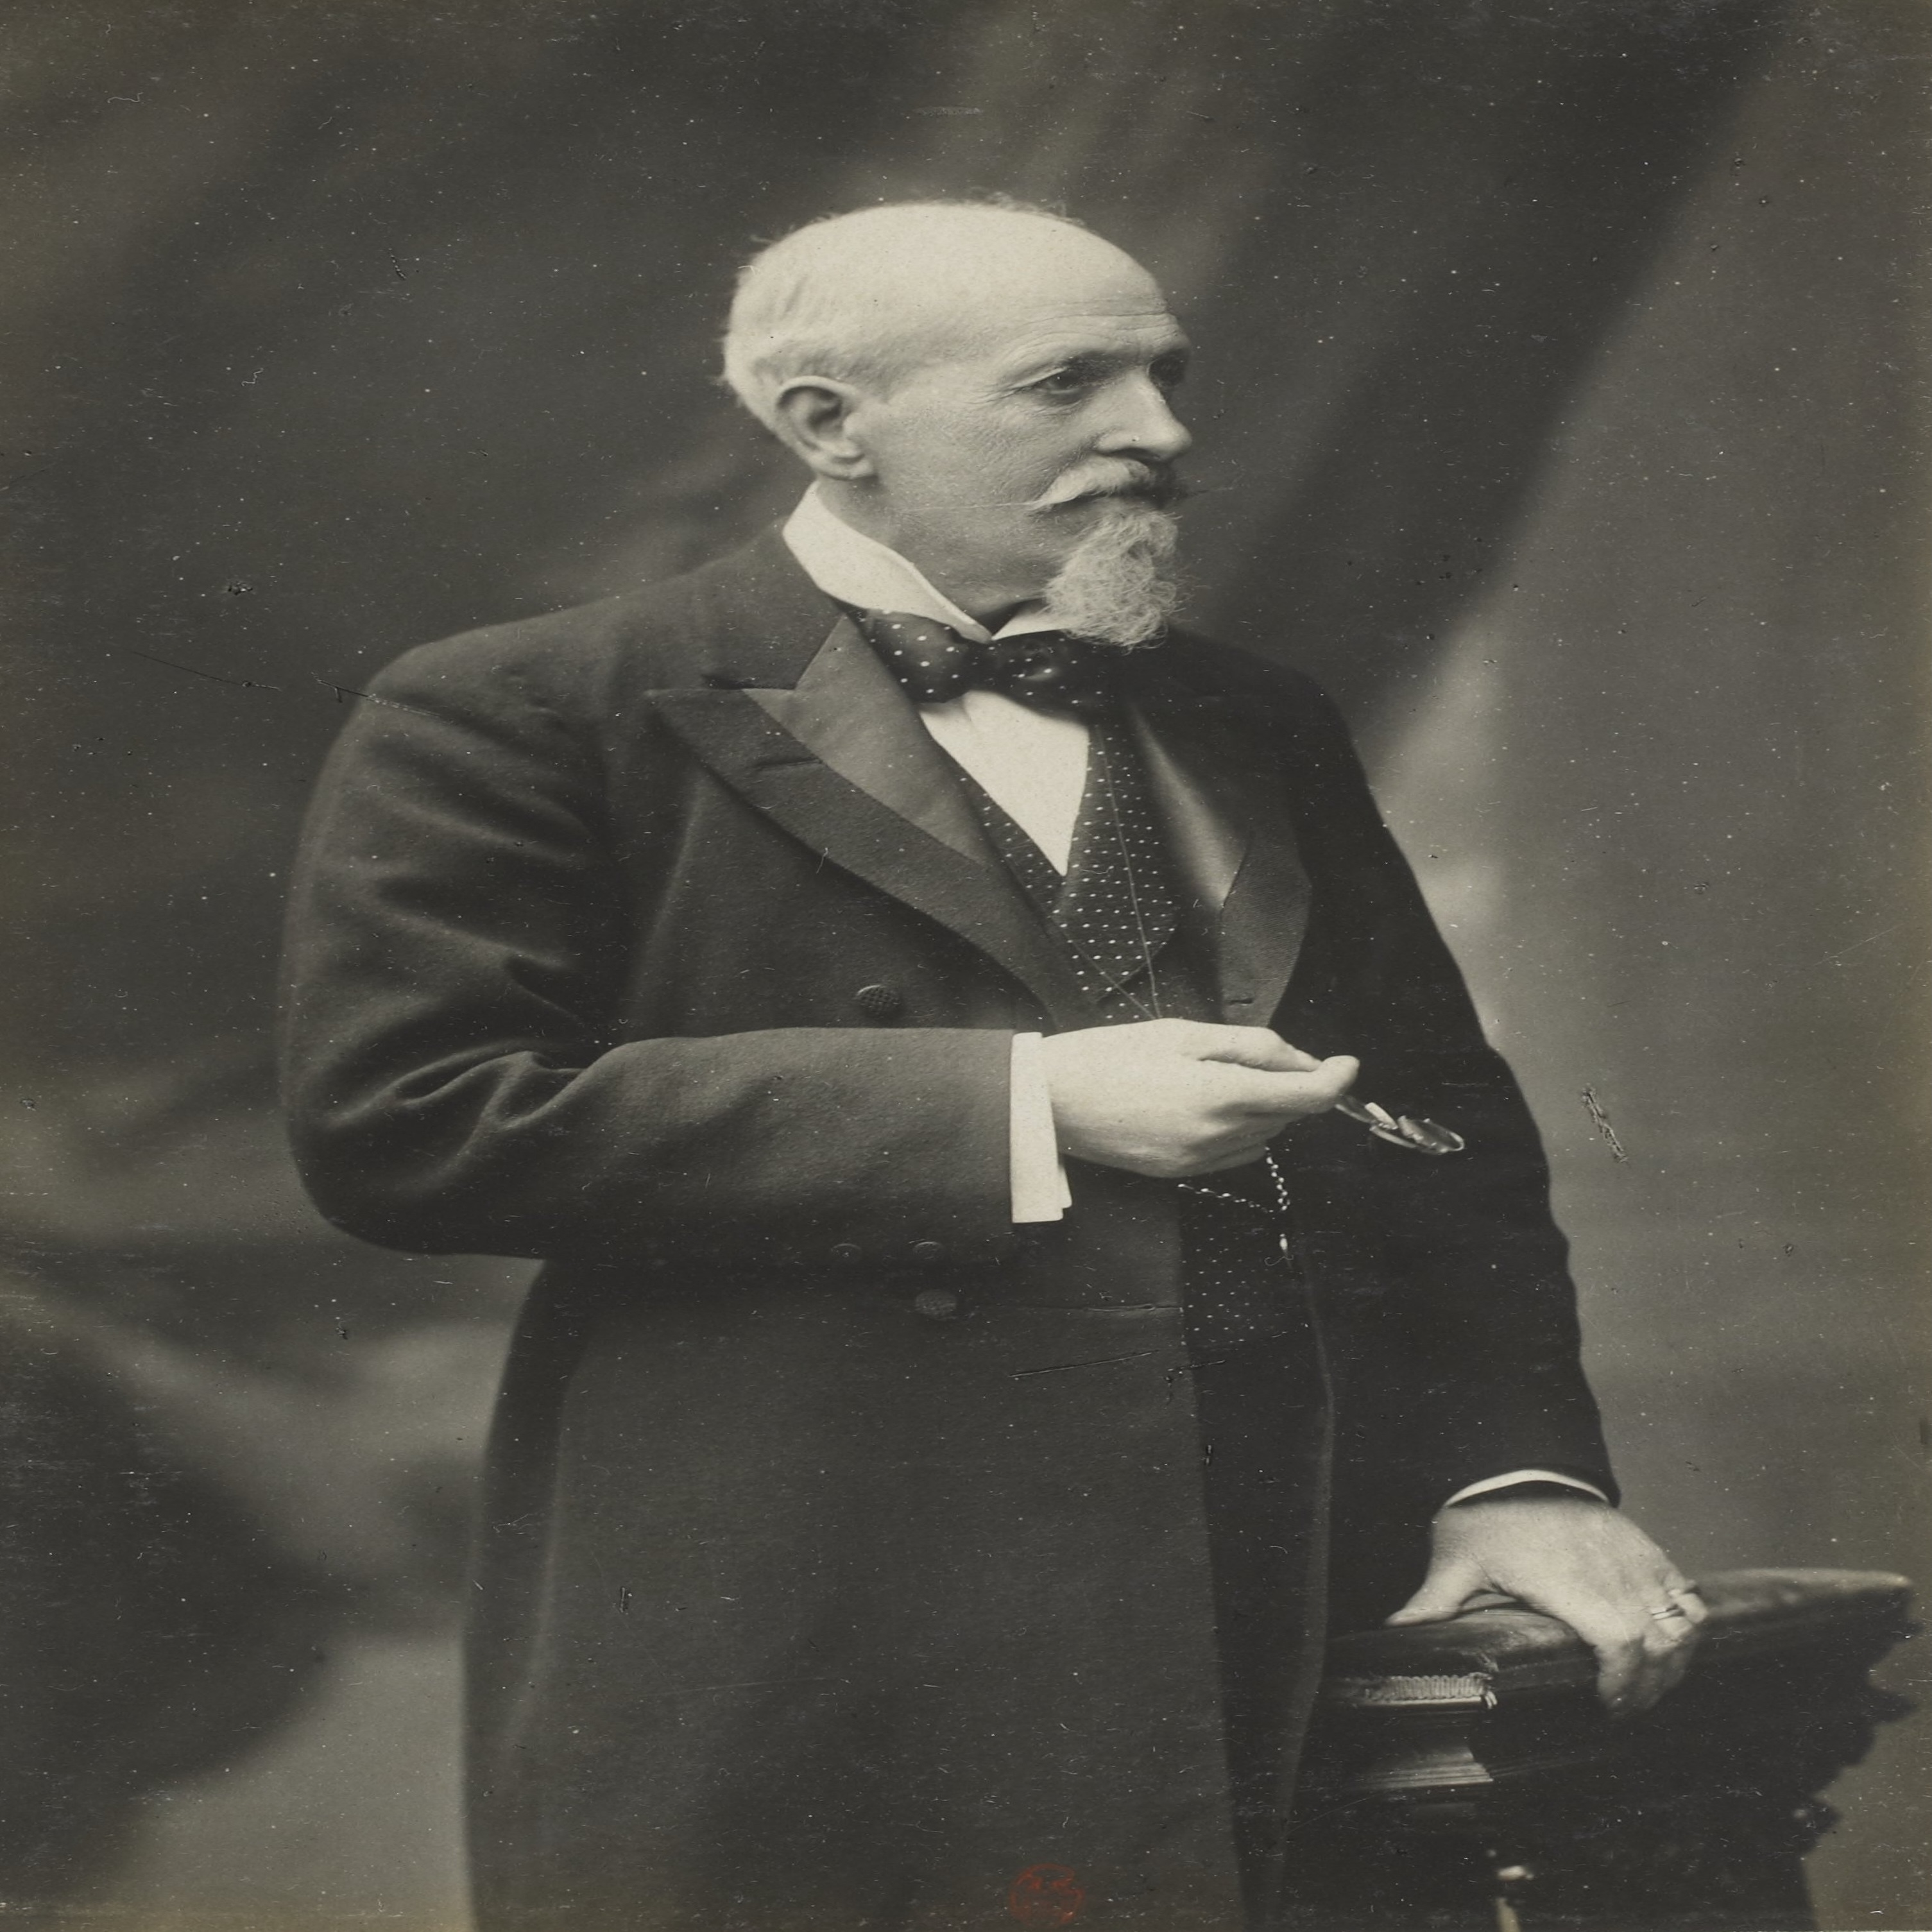
\includegraphics[width=\linewidth]{spea.jpg}
    \end{figure}
    \column{0.25\textwidth}
    \begin{figure}
        \centering
        \footnotesize\textbf{Louis Thurstone} \\
        \vspace{0.2em}
        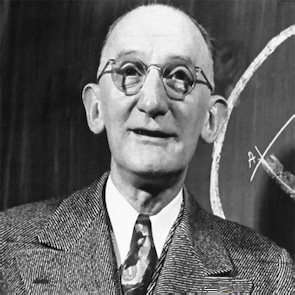
\includegraphics[width=\linewidth]{_thurstone.jpg}
    \end{figure}
    \column{0.25\textwidth}
    \begin{figure}
        \centering
        \footnotesize\textbf{Karl Jöreskog} \\
        \vspace{0.2em}
        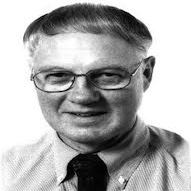
\includegraphics[width=\linewidth]{_joreskog.jpg}
    \end{figure}
  \end{columns}
\end{frame}

\begin{frame}{Breve storia della SEM}
    \begin{block}{CB-SEM: Covariance-Based SEM}
        \begin{itemize}
            \item Formalizzato da Karl Jöreskog (1969) con LISREL;
            \item Obiettivo: riprodurre la \textbf{matrice di covarianze} osservata;
            \item Basato sulla \textbf{massima verosimiglianza}.
        \end{itemize}
    \end{block}
    \begin{block}{PLS-SEM: Partial Least Squares SEM}
        \begin{itemize}
            \item Introdotto da Herman Wold (anni '70);
            \item Approccio \textbf{component-based}, iterativo;
            \item Focalizzato sulla \textbf{massimizzazione della varianza spiegata};
            \item Preferibile in caso di: piccoli campioni, modelli formativi, non-normalità.
        \end{itemize}
    \end{block}
\end{frame}

\section{Un po' di teoria}
\begin{frame}{Processo di analisi}
    L'analisi SEM passa attraverso quattro fasi, uguali per \textbf{CB-SEM} e \textbf{PLS-SEM}. Tuttavia, i criteri specifici da utilizzare differiscono, in quanto questi modelli differiscono per funzionamento e per scopi di utilizzo (es. VL Riflessive o Formative). Ci soffermeremo sulle quattro fasi del processo con un focus sul \textbf{CB-SEM}: \\
    \vspace{1em}
    \begin{enumerate}
        \item Specifica del modello
        \item Identificazione del modello
        \item Stima del modello
        \item Valutazione del modello
    \end{enumerate} 
\end{frame}

\begin{frame}{Specifica del modello}
    \begin{block}{Fase 1:}
        La prima fase consiste nel definire il modello teorico e le relazioni ipotizzate. In molti software (compreso Stata) la specifica del modello può avvenire sia attraverso il disegno di diagrammi, sia attraverso la scrittura di codice. \\
        \vspace{1em}
        \centering
        \begin{tikzpicture}
            \node[lv] (et) {$\eta$};
            \node[lv, left=2 of et] (xi) {$\xi$};
            \node[mv, left=of xi] (x2) {$x_2$};
            \node[mv, above=of x2] (x1) {$x_1$};
            \node[mv, below=of x2] (x3) {$x_3$};
            \node[mv, right=of et] (y2) {$y_2$};
            \node[mv, above=of y2] (y1) {$y_1$};
            \node[mv, below=of y2] (y3) {$y_3$};
            \draw[arrow] (xi) -- (et);
            \draw[arrow] (xi) -- (x1);
            \draw[arrow] (xi) -- (x2);
            \draw[arrow] (xi) -- (x3);
            \draw[arrow] (et) -- (y1);
            \draw[arrow] (et) -- (y2);
            \draw[arrow] (et) -- (y3);
        \end{tikzpicture} \\
        \vspace{1em}
        \small
        \texttt{. sem (Xi -> x1 x2 x3) (Eta -> y1 y2 y3) (Xi -> Eta)}
    \end{block}
\end{frame}

\begin{frame}{Identificazione del modello}
    \begin{block}{Fase 2:}
        Purtroppo, non tutto quello che si può disegnare si può anche stimare. La \textbf{T-Rule}, ad esempio, è una condizione necessaria (ma non sufficiente) affinché un modello sia identificabile:
    \end{block}
    \[
    t \leq \frac{p(p+1)}{2}
    \]
    \begin{itemize}
        \item $t$ è il numero di parametri da stimare (frecce nei diagrammi);
        \item $p$ è il numero di variabili manifeste del modello.
    \end{itemize}
    \vspace{1em}
    \small
    \begin{itemize}
        \item Se $t < \frac{p(p+1)}{2}$ il modello è \textit{over-identified}: stimabile e testabile;
        \item Se $t = \frac{p(p+1)}{2}$ il modello è \textit{just-identified}: stimabile ma non testabile (gradi di libertà = 0);
        \item Se $t > \frac{p(p+1)}{2}$ il modello è \textit{under-identified}: non stimabile in modo univoco.
    \end{itemize}
\end{frame}

\begin{frame}{Identificazione del modello}
    \centering
    $t \leq \frac{p(p+1)}{2}$ \hspace{1em} \textbf{?} \\
    \vspace{2em}
        \begin{tikzpicture}
            \node[lv] (l) {$\eta$};
            \node[mv, left=of l] (x2) {$y_2$};
            \node[mv, above=of x2] (x1) {$y_1$};
            \node[mv, below=of x2] (x3) {$y_3$};
            \draw[arrow] (l) -- (x1);
            \draw[arrow] (l) -- (x2);
            \draw[arrow] (l) -- (x3);
            \pause
            \node[ev, left=of x1] (e1) {$\varepsilon_1$};
            \node[ev, left=of x2] (e2) {$\varepsilon_2$};
            \node[ev, left=of x3] (e3) {$\varepsilon_3$};
            \draw[arrow] (e1) -- (x1);
            \draw[arrow] (e2) -- (x2);
            \draw[arrow] (e3) -- (x3);
        \end{tikzpicture}
\end{frame}

\begin{frame}{Stima del modello}
    \begin{block}{Fase 3:}
        La stima del modello consiste nel calcolare i valori dei parametri che meglio riproducono la matrice di covarianze osservata (tipicamente attraverso \textit{massima verosimiglianza}).
    \end{block}
\end{frame}

\begin{frame}{Valutazione del modello}
    \begin{block}{Fase 4:}
        La valutazione del modello avviene su tre livelli:
        \begin{enumerate}
            \item \textbf{Bontà di adattamento globale}:
            \begin{itemize}
                \item $\chi^2$ test (meglio non significativo)
                \item RMSEA $< 0.06$
                \item CFI, TLI $> 0.95$
                \item SRMR $< 0.08$
            \end{itemize}
            \item \textbf{Modello di misurazione}:
            \begin{itemize}
                \item $\lambda_i$ (carichi fattoriali) $> 0.5$ e significativi
                \item CR (Composite Reliability) $> 0.7$
                \item AVE (Average Variance Extracted) $> 0.5$
                \item Discriminant validity (es. criterio di Fornell-Larcker)
            \end{itemize}
            \item \textbf{Modello strutturale}:
            \begin{itemize}
                \item $\beta$ (path coeff.) significativi
                \item $R^2$ accettabili per le endogene
                \item Effetti diretti, indiretti e totali significativi (se rilevante)
            \end{itemize}
        \end{enumerate}
    \end{block}
\end{frame}

\begin{frame}{Modification Indices}
    \begin{block}{Cosa sono?}
        I \textbf{Modification Indices} (MI) segnalano potenziali miglioramenti al modello introducendo parametri non specificati (es. covarianze residue).
    \end{block}
    \vspace{1em}
    \textbf{Attenzione:} le modifiche suggerite vanno accettate solo se teoricamente giustificate, per evitare \textit{overfitting}.\\
    \vspace{1em}
    Introducendo nuovi parametri da stimare, ripartiamo dalla Fase 1!
\end{frame}

\section{Un po' di Stata}
\begin{frame}{clear all ;)}
    \texttt{. webuse set data.califano.xyz} \\
    \texttt{. webuse mamme}
\end{frame}

\end{document}
